\documentclass[a4paper, 12pt]{article}
\usepackage[utf8]{inputenc}
\usepackage[T1, T2A]{fontenc}
\usepackage[a4paper, top=2cm, bottom=2cm, left=1cm, right=1cm, marginparwidth=1.75cm]{geometry}
\usepackage{graphicx}
\usepackage{amsmath}
\usepackage{indentfirst}
\usepackage[english, russian]{babel}
\usepackage[section,above,below]{placeins}
\usepackage[noend]{algorithmic}
\usepackage{amssymb}
\usepackage{amsfonts}
\usepackage{pdfpages} 


\newcommand{\jone}[1]{\frac{\partial J_0(\alpha r)}{\partial #1}}
\newcommand{\jtwo}[1]{\frac{\partial^2 J_0(\alpha r)}{\partial #1^2}}
\newcommand{\jxy}{\frac{\partial^2 J_0(\alpha r)}{\partial x \partial y}}
\newcommand{\ww}{\omega}
\newcommand{\dw}{\Delta \omega}

\begin{document}

\section{Описание задачи}
{\bf Постановка задачи}. Рассматриваются гармонические колебания изотропного слоя толщины $h$,
занимающего в системе координат $(x, y, z)$ полубесконечную область
$D: \{ -\infty< x,y<\infty, -h \leq z \leq 0 \}$.
Источником колебаний служит тонкий вертикально поляризованный пьезоактуатор,
контактирующий с поверхностью $z = 0$ по области $\Omega$ с
центром в начале координат.
С использованием принципа суперпозиции и обратного преобразования Фурье
$\mathcal{F}_t^{-1}$ нестационарные перемещения слоя ${\bf u}({\bf x},t)$
могут быть выражены через гармонические ${\bf u}({\bf x},\omega)e^{-i \omega t}$ (частотный спектр),
причём комплексная амплитуда перемещений ${\bf u}({\bf x},\omega)=\{u_x,u_y,u_z \}$
удовлетворяет уравнению Ляме:
\begin{equation}
    \mathcal{L} {\bf u}+ \rho \omega^2 {\bf u}=0,
\end{equation}
где $\mathcal{L}$ --- оператор Ляме:
\begin{equation*}
    \mathcal{L} {\bf u}=(\lambda+2\mu){\bf u}+\mu \Delta {\bf u},
\end{equation*}
$\lambda, \mu$ --- константы Ляме.

Внешние поверхности волновода $z=0$ и $z=-h$ предполагаются свободными от напряжений
${\bf \tau}=\{\tau_{xz}, \tau_{yz}, \sigma_z \}$ за исключением области $\Omega$,
где действие актуатора моделируется нагрузкой ${\bf q}$. С использованием полуаналитического интегрального подхода получаем, что
поле ${\bf u}$, возбуждаемое пьезоактуатором в волноводе без препятствий (поле источника), при фиксированной частоте $\omega$ представимо в виде
\begin{equation}
    {\bf u}({\bf x})= \iint_{\Omega} k({\bf x}-{\bf \zeta}) {\bf q}({\bf \zeta}) d {\bf \zeta}=
    \dfrac{1}{4 \pi^2} \int_{\Gamma_1}\int_{\Gamma_2} K(\alpha_1,\alpha_2,z) Q(\alpha_1,\alpha_2) e^{-i (\alpha_1 x+ \alpha_2 y)} d\alpha_1 d\alpha_2,
\label{u1}
\end{equation}
где $K(\alpha_1,\alpha_2,z)$ и $Q(\alpha_1,\alpha_2)$ --- Фурье-символы матрицы Грина $k({\bf x})$
для слоистой упругой среды с заданными на поверхности $z=0$ напряжениями и нагрузки ${\bf q}({\bf x})$ соответственно.

Матрица $K$ представима в следующем виде:
\begin{equation}
    K(\alpha_1, \alpha_2,z)=
\begin{pmatrix} 
    -i\left( M \alpha_1^2 +N \alpha_2^2\right)/\alpha^2 & -i(M-N)\alpha_1 \alpha_2 /\alpha^2&-iP\alpha_1\\ 
    -i(M-N)\alpha_1 \alpha_2 /\alpha^2& -i\left( M \alpha_2^2 +N \alpha_1^2\right) /\alpha^2&-iP\alpha_2\\
    S\alpha_1 /\alpha^2&S\alpha_2 /\alpha^2& R \\
\end{pmatrix},
\label{K1}
\end{equation}
где $\alpha^2=\alpha_1^2+\alpha_2^2, P,R,M,S,N$ --- некоторые комплексные функции, зависящие от $\alpha$ и $z$.
Алгоритм их построения приводится в работах \cite{g89,g90}. Конкретно для слоя конечной толщины получаем: $P=v_1 \cdot e_1$, $R=v_1 \cdot e_2$, $M=v_2 \cdot e_1$, $S=v_2 \cdot e_2$ и
$N=\frac{i \ch (\sigma_2(z+h))}{\mu \sigma_2 \sh(\sigma_2 h)}$,
\begin{equation*}
    e_1=(\exp(\sigma_1 h),\exp(-\sigma_1(z+h)), \sigma_2 \exp(\sigma_2 z), -\sigma_2\exp(-\sigma_2(z+h))),
\end{equation*}
\begin{equation*}
    e_2=(\sigma_1 \exp(\sigma_1 h),-\sigma_1 \exp(-\sigma_1(z+h)), \alpha^2 \exp(\sigma_2 z), \alpha^2 \exp(-\sigma_2(z+h))),
\end{equation*}
\begin{equation*}
    \sigma_i=\sqrt{\alpha^2 - \kappa^2_i}, \kappa^2_1=\dfrac{\rho \omega^2}{2\mu+\lambda},\kappa^2_2=\dfrac{\rho \omega^2}{\mu},
\end{equation*}
$\rho$ -- плотность материала, $v_1,v_2$ -- первые два столбца матрицы $A^{-1}$, где

\begin{equation*}
     A = 
    \begin{pmatrix}
        a & a\exp(-\sigma_1 h) & c & -c \exp(-\sigma_2 h)\\
        -b & b\exp(-\sigma_1 h) & d & d \exp(-\sigma_2 h)\\
        a \exp(-\sigma_1 h)& a & c\exp(-\sigma_2 h) & -c \\
        -b \exp(-\sigma_1 h) & b& d\exp(-\sigma_2 h)& d\\
    \end{pmatrix},    
\end{equation*}
в которой $a=2\mu (\alpha^2 - \frac{1}{2} \kappa^2_2), b= 2\mu \sigma_1 i, c= 2\mu \sigma_2 \alpha^2, d= - 2\mu i \cdot a$.

{\bf Переход к полярным координатам}. Поскольку указанные функции зависят только от переменной $\alpha$ (а не отдельно от $\alpha_1,\alpha_2$),
интеграл (\ref{u1}) можно свести к однократному.
Для этого осуществляется переход в полярную систему координат (\cite{g89}),
что позволяет после некоторых преобразований представить равенство (\ref{u1}) в виде:
\begin{multline}
    {\bf u}(x,y,z)=\frac{1}{2\pi}\iint_{-\infty}^{\infty}K(\alpha_1,\alpha_2,z)Q(\alpha_1,\alpha_2)e^{-i(\alpha_1 x+\alpha_2 y)}d\alpha_1 d\alpha_2=\\
    =\frac{1}{2\pi}\int_{\Gamma^+}(K*J)(\alpha, x,y,z)Q(\alpha)\alpha d\alpha=\frac{1}{2\pi}\int_{\Gamma^+}(K*J*\alpha)(\alpha, x,y,z)Q(\alpha) d\alpha,
\label{u2}
\end{multline}
где
\begin{multline}
    (K*J*\alpha)(\alpha, x,y,z)=
\begin{pmatrix} 
    i\left( M \jtwo{x} +N \jtwo{y}\right)\frac{1}{\alpha} & i(M-N)\jxy\frac{1}{\alpha} &P\jone{x}\alpha\\ 
    i(M-N)\jxy\frac{1}{\alpha}& i\left( M \jtwo{y} +N \jtwo{x}\right)\frac{1}{\alpha} &P\jone{y}\alpha\\
    iS\jone{x}\frac{1}{\alpha}&iS\jone{y}\frac{1}{\alpha} & R J_0(\alpha r)\alpha\\
\end{pmatrix}
\label{KJ}
\end{multline}
и производные функций Бесселя с учётом соотношения
\begin{equation}
    J_{\nu}'(z)=\frac{\nu}{z}J_{\nu}(z)-J_{\nu+1}(z)=J_{\nu-1}(z)-\frac{\nu}{z}J_{\nu}(z)
\end{equation}
получаются:
\begin{equation}
    \jone{x}=-J_1(\alpha r)\frac{\alpha x}{r},
\end{equation}
\begin{equation}
    \jone{y}=-J_1(\alpha r)\frac{\alpha y}{r},
\end{equation}
\begin{equation}
    \jtwo{x}=-\frac{\alpha}{r^2}\left(\alpha J_0(\alpha r)x^2- \frac{1}{r} J_1(\alpha r)(x^2-y^2)\right),
\end{equation}
\begin{equation}
    \jtwo{y}=-\frac{\alpha}{r^2}\left(\alpha J_0(\alpha r)y^2- \frac{1}{r} J_1(\alpha r)(y^2-x^2)\right),
\end{equation}
\begin{equation}
    \jxy=-\frac{\alpha xy}{r^2}\left(\alpha J_0(\alpha r) - 2\frac{J_1(\alpha r)}{r}\right).
\end{equation}
Контур $\Gamma^+$ в уравнении (\ref{u2}) представляет собой положительную действительную полуось с отклонением в соответствии с принципом предельного поглощения (\cite{TS})
таким образом, чтобы обходить полюса функции $K*J*\alpha$ (уравнение \ref{KJ}) снизу.

{\bf Представление u через вычеты}. Наряду с прямым вычислением интеграла (\ref{u2}) в дальней от источника зоне
(т.е. при $r \gg \text{diam } \Omega$) использовались соответствующие асимптотические представления
(\cite{g89}), полученные с применением теории вычетов. В результате
\begin{multline}
    {\bf u}(x,y,z)=\frac{i}{2} \sum_{\zeta} \bar{K}(\zeta) Q(\zeta) \approx \\
    \frac{i}{2} \sum_{\zeta} \frac{\varepsilon}{2} \left( (K*J*\alpha)(\zeta+\varepsilon,x,y,z)-(K*J*\alpha)(\zeta-\varepsilon,x,y,z) \right)  Q(\zeta),
\label{resU}
\end{multline}
где $\zeta$ --- полюса функции $K*J*\alpha$, $\varepsilon$ --- некоторая погрешность, большая погрешности поиска полюсов,
$\bar{K}(\zeta_i)$ --- вычет функции $K*J*\alpha$ в полюсе $\zeta_i$.

{\bf Вид функции q}. Поскольку в области низких частот нагрузка ${\bf q}$ концентрируется в основном на границе пьезоэлемента,
допустима аппроксимация ${\bf q}$ по нормальным модам, центрированным на точечных источниках ${\bf x}_j$, в следующем виде (\cite{eng}):
\begin{equation}
    {\bf q}({\bf x}) \approx \sum_{j=1}^{N_q} p_j \delta({\bf x}-{\bf x}_j)
    \begin{pmatrix}
        \cos \varphi_j\\
        \sin \varphi_j\\
        0
    \end{pmatrix}=
    \sum_{j=1}^{N_q} {\bf q}_j
\end{equation}
где $N_q$ --- число точечных источников, ${\bf x}_j$ --- координата $j$-го источника (располагается на границе пьезоэлемента), $p_j$ --- весовой коэффициент,
$\varphi_j$ --- угол между осью $X$ и нормалью к ${\bf x}_j$ от центра пьезоэлемента,
$\delta$ --- дельта-функция, определяемая соотношением:
\begin{equation*}
    2 \pi \int_0^{\infty} f(r) \delta(r-a) r dr =f(a).
\end{equation*}

В таком случае для функции ${\bf u}$ из уравнения (\ref{u1}) верно:
\begin{equation}
    {\bf u}({\bf x}) \approx \sum_{j=1}^{N_q} {\bf u}_j({\bf x})=\sum_{j=1}^{N_q} k({\bf x}-{\bf x}_j) {\bf q}_j,
\end{equation}
где ${\bf u}_j({\bf x})$ --- такая же функция из (\ref{u2}) или (\ref{resU}) с той разницей, что $r=r_j=|{\bf x} -{\bf x}_j|$.


\section{Сравнение вычетов и интегралов}
При численной реализации интегралы типа (\ref{u2}) считались по квадратурам Гаусса-Кронрода,
кривая $\Gamma^+$ совпадала с лучом $(0,\infty)$ везде, кроме отрезка $[\frac{1}{2} \min \{\zeta_i\}, \frac{3}{2} \max \{\zeta_i\}]$,
где $\{\zeta_i \}$ --- множество положительный вещественных полюсов подынтегральной функции,
искавшихся на достаточно большом отрезке в качестве корней уравнения $\Delta(\alpha)=\Delta(\alpha,\omega)=0$, в котором $\Delta$ --- общий знаменатель функций $P,R,M,S,N$.
На самом отрезке $[\frac{1}{2} \min \{\zeta_i\}, \frac{3}{2} \max \{\zeta_i\}]$ контур $\Gamma^+$ деформировался в нижнюю комплексную полуплоскость.
При подсчёте искомой функции по формуле (\ref{resU}) сумма бралась по всем положительным вещественным полюсам $\Delta$.
Расчёты проводились для поверхности пластины ($z=0$).

Интерес представляли функции $u_z=u_z(x,y,z), u_r= u_x \cos \varphi + u_y \sin \varphi$,
где $\varphi$ --- угол между осью $X$ и нормалью к ${\bf x}$ от центра пьезоэлемента.
На рисунках показано, как функции $u_z, u_r$, посчитанные по вычетам, аппроксимируют те же функции, посчитанные через интегралы.

\begin{figure}[h]
    \begin{minipage}[h]{0.49\linewidth}
    \center{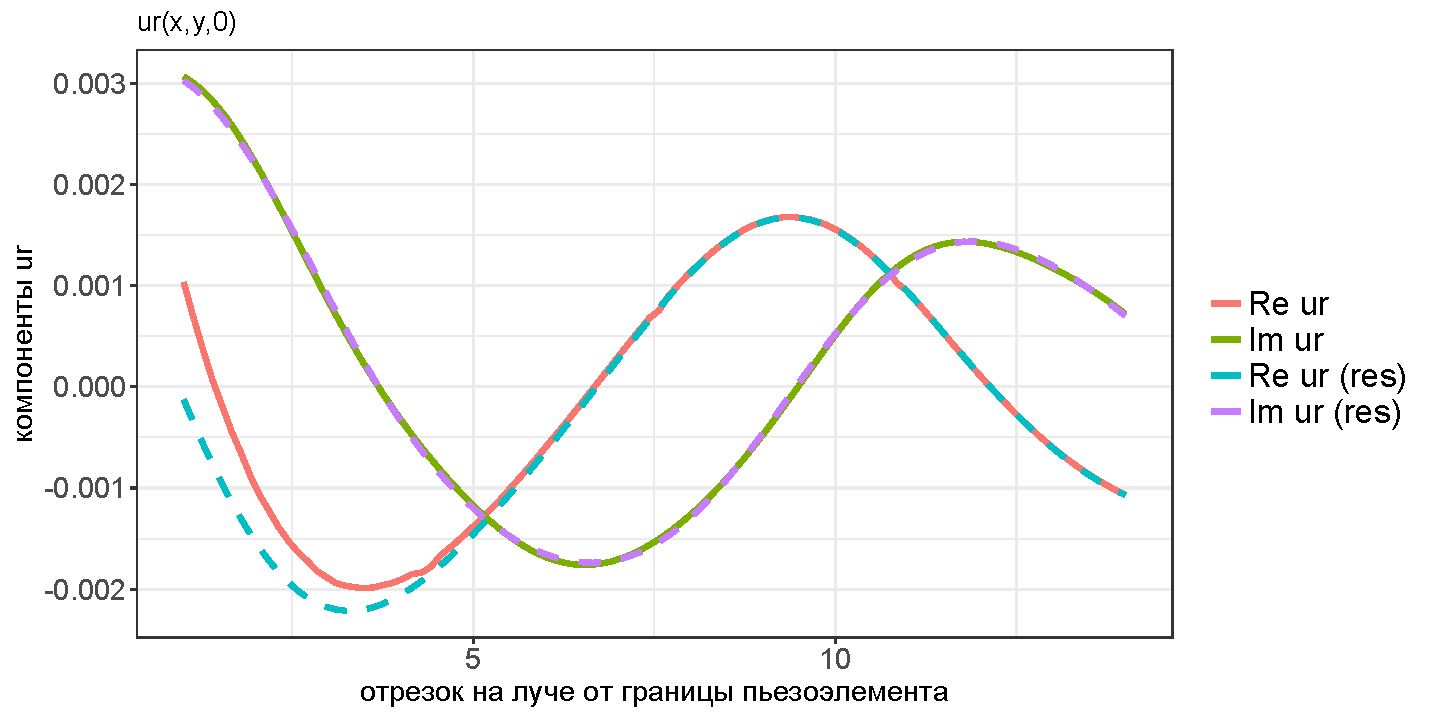
\includegraphics[width=\linewidth]{url.pdf} \\ а)}
    \end{minipage}
    \hfill
    \begin{minipage}[h]{0.49\linewidth}
    \center{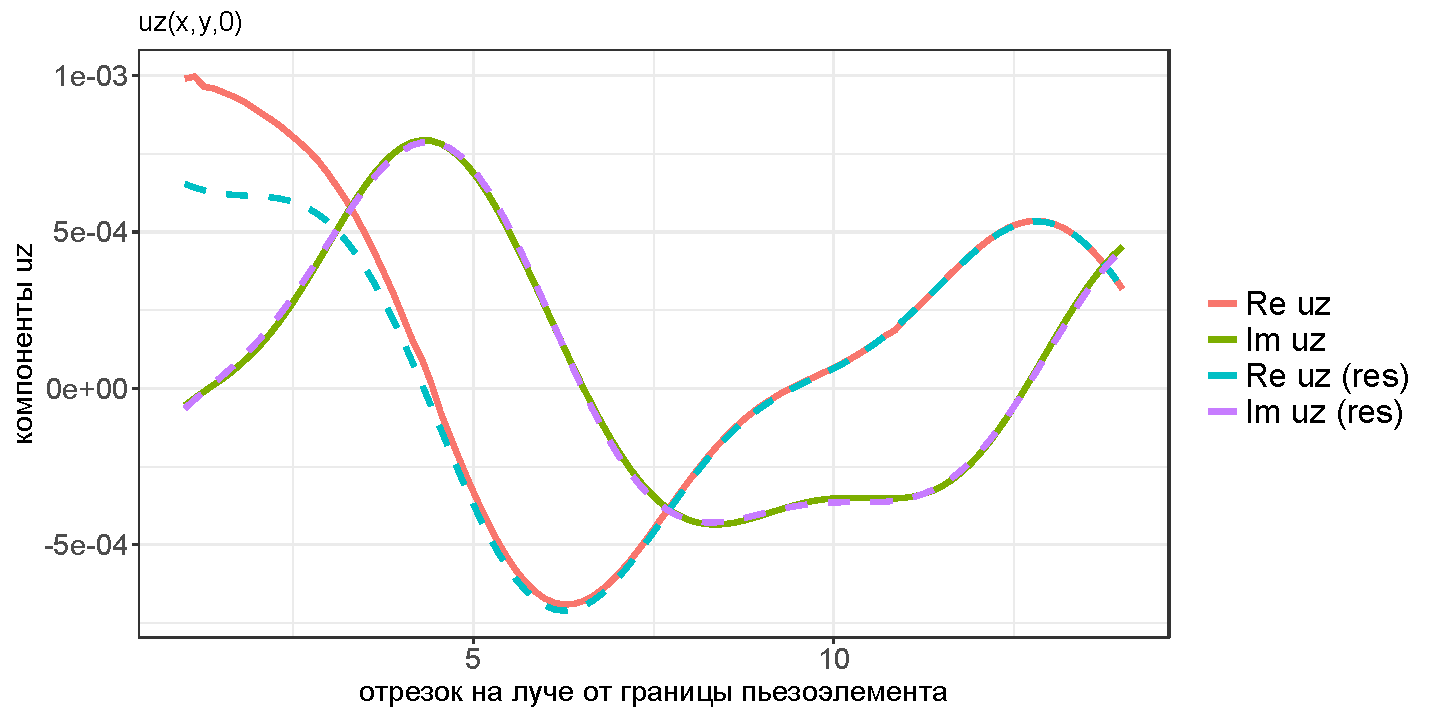
\includegraphics[width=\linewidth]{uzl.pdf} \\ б)}
    \end{minipage}
    \caption{Действительная и мнимая части функций $u_z, u_r$, посчитанных через интегралы и по вычетам, при удалении от пьезоэлемента по нормали. Центр пьезоэлемента --- $(1; 1)$, радиус $r=3$, угол наклона $\varphi= \frac{\pi}{6}$, частота $\omega =3$, число источников $N_q=80$.}
    \label{resl}
    \end{figure}


\section{Сравнение двух моделей точечных источников}
Искомое возмущение аппроксимируется моделью касательных точечных сил. Ввиду особенностей пьезоактуатора (Рис. \ref{act1}) имеется два варианта расстановки точечных источников: по внешней окружности и по внутреннему полумесяцу (Рис. \ref{act2}). Технически вся разница заключается в координатах точек приложения нормалей, в направлении некоторых нормалей и в количестве точечных источников, необходимых для достижения требуемой точности аппроксимации, однако вариант с загнутым электородом лучше повторяет поведение искомой функции на "средних" дистанциях от источника (Рис. \ref{act3}) 
\begin{figure}[h]   
    \center{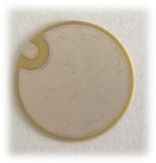
\includegraphics[width=0.4\linewidth]{act.png}}
    \caption{Фотография пьезоактуатора}
    \label{act1}
\end{figure}
\begin{figure}[h]   
    \center{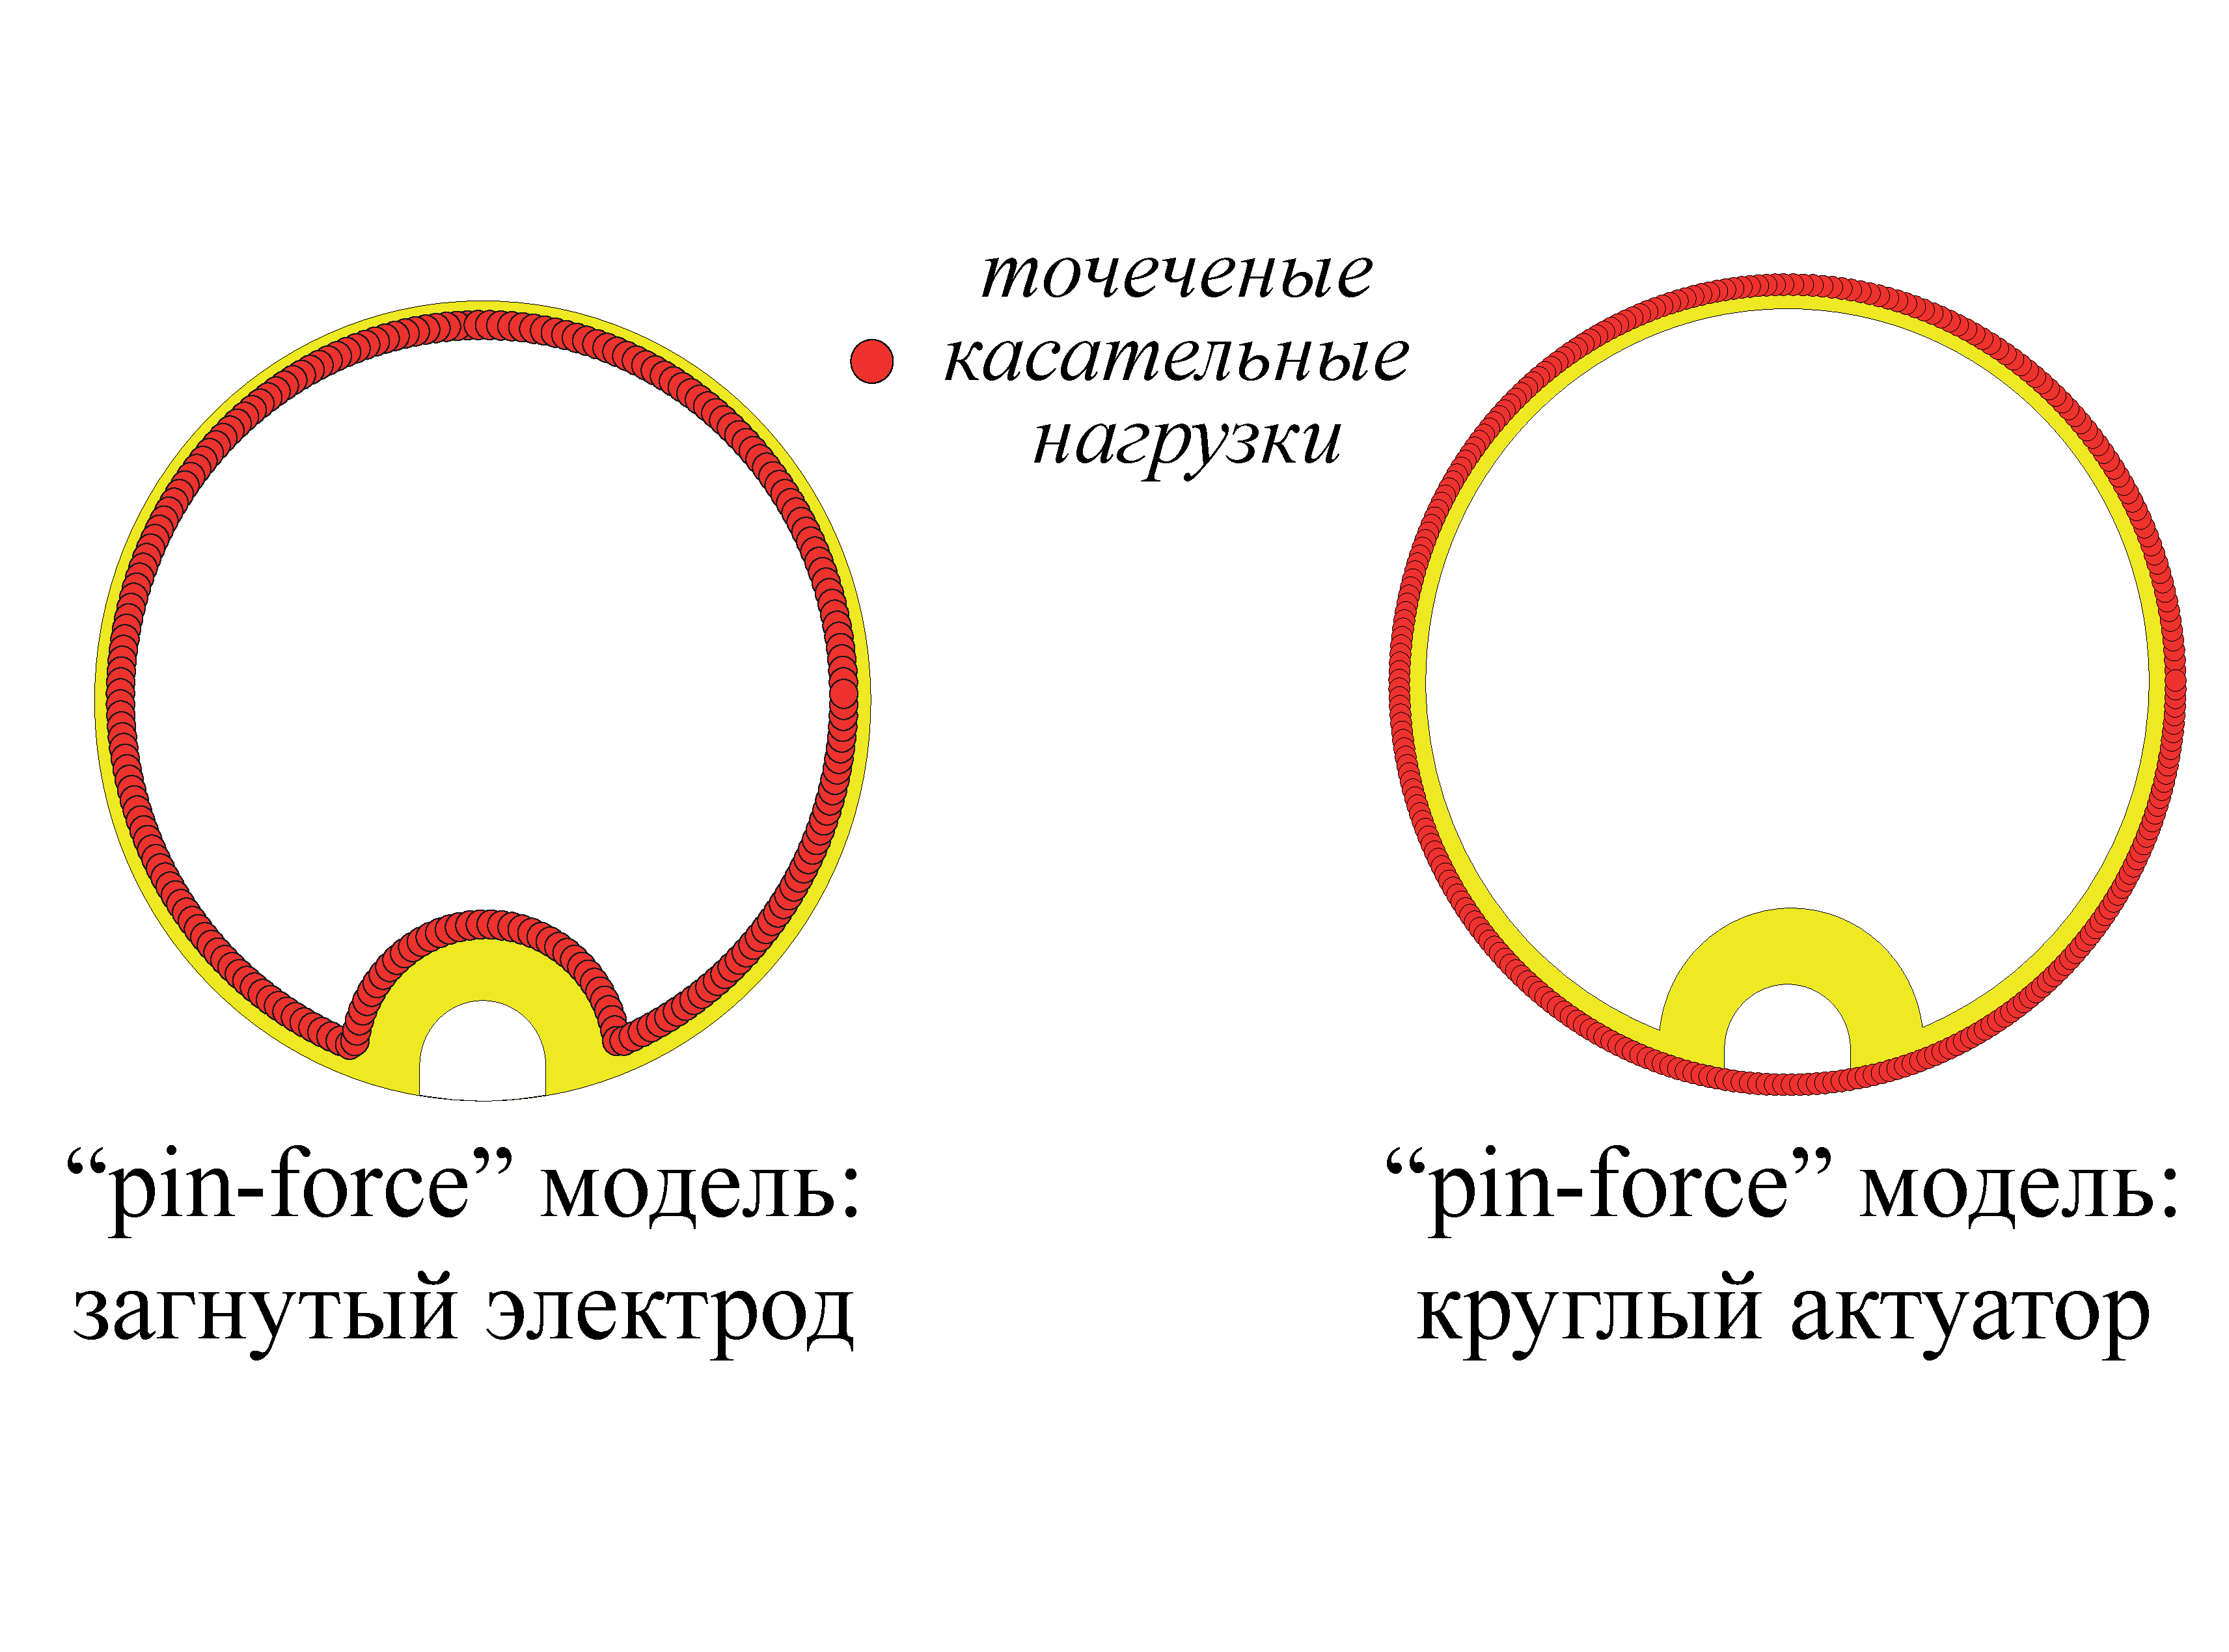
\includegraphics[width=0.7\linewidth]{act2.pdf}}
    \caption{Варианты расстановки точечных источников}
    \label{act2}
    \end{figure}
    \begin{figure}[h]   
        \center{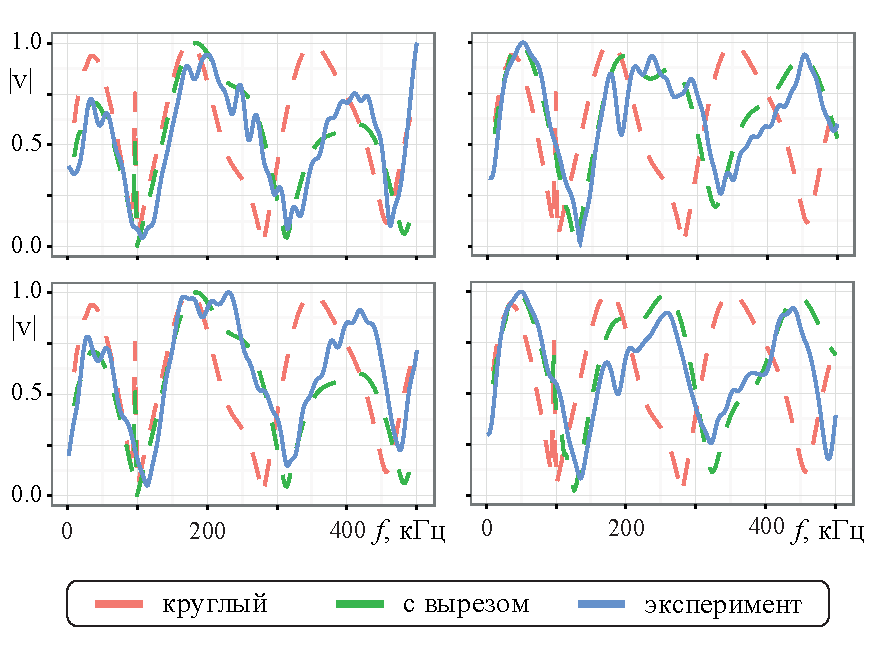
\includegraphics[width=0.9\linewidth]{4my.pdf}}
        \caption{Что-то там в разных точках}
        \label{act3}
    \end{figure}



\section{Общая схема эксперимента}
Изучаемый образец представляет собой пластину сплава АМг2М толщиной 2мм, размером 1000мм на 500мм. В качестве источника колебаний к образцу приклеены тонкие пьезоактивные элементы, далее обозначаемые ПЭ, размера 16мм в диаметре, 0.25мм толщиной изготовленные из материала Pic151 и размещенные в координатах (450,150), (450,350), (450,550), (650,150), (650,350), (650,550) (рисунок \ref{dats}) считая от левого нижнего угла в мм.
\begin{figure}[h]
    \center{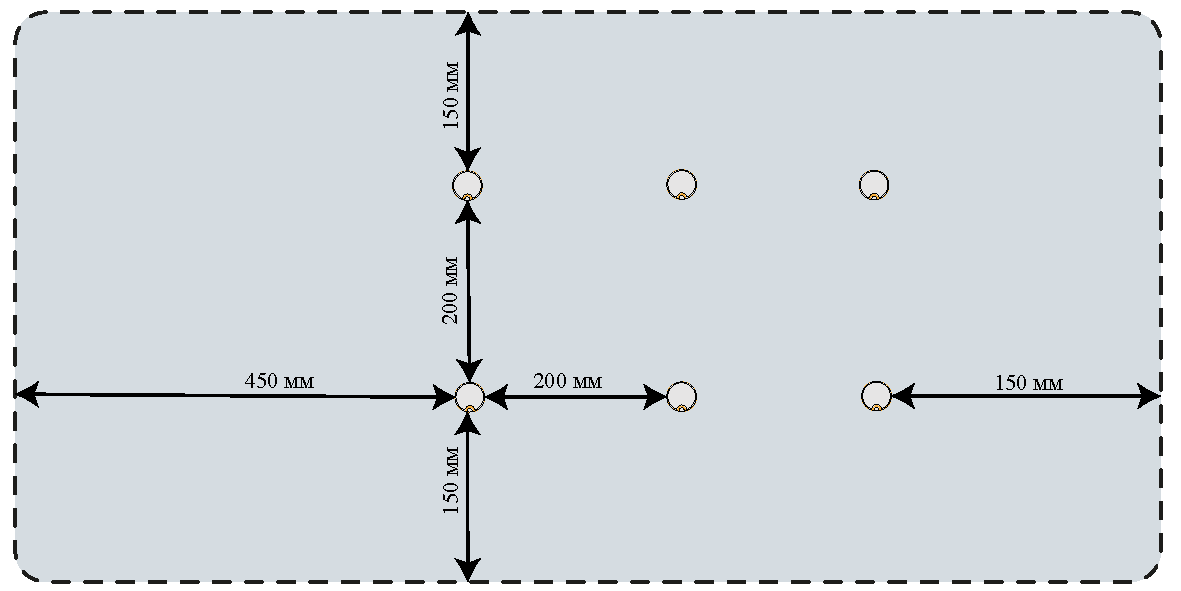
\includegraphics[width=0.8\linewidth]{dats.pdf}}
    \caption{Схема расположения датчиков}
    \label{dats}
\end{figure}
Для возбуждения колебаний на пьезоэлементы подается нестационарное электрическое напряжение в форме тональных посылок $f(t)$ подается сигнал с центральной частотой 100 КГц (рисунок \ref{window}).

    \begin{figure}[h]
        \center{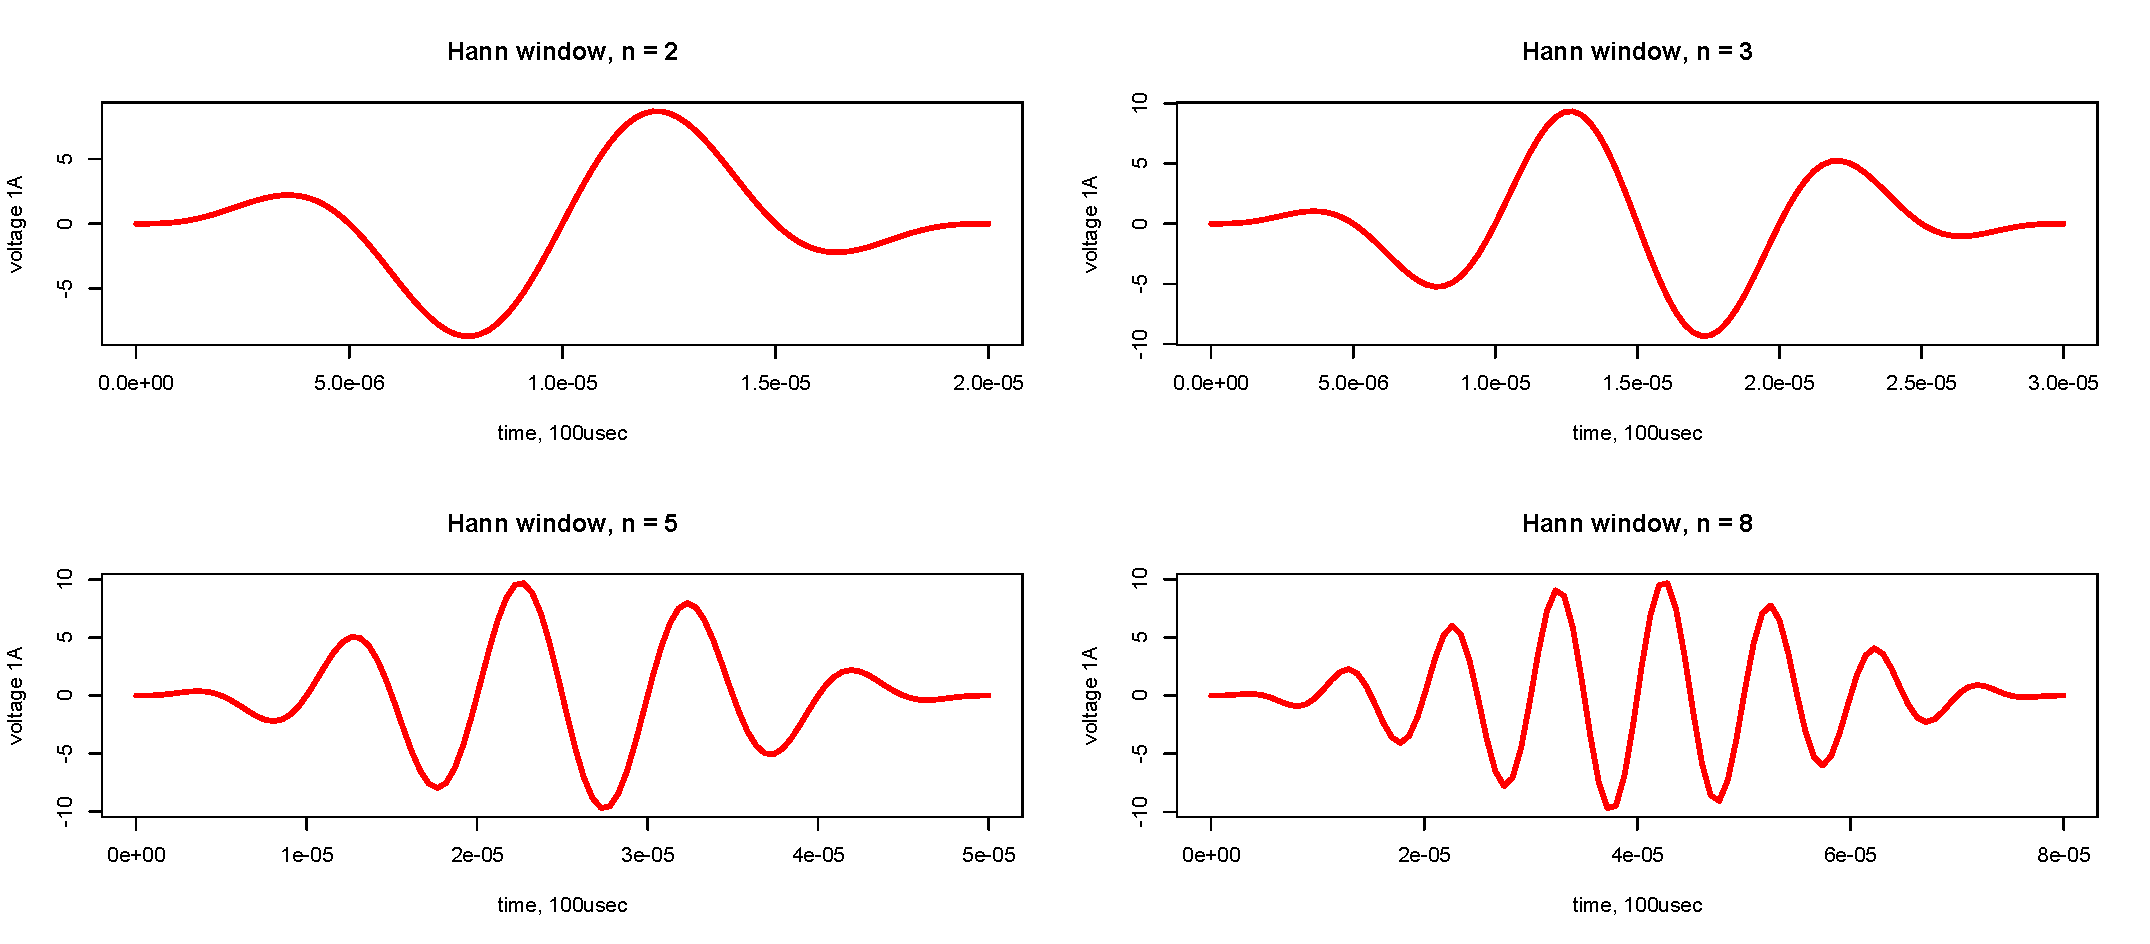
\includegraphics[width=0.9\linewidth]{wind.pdf}}
        \caption{Функция $f(t)=10 \sin (2\pi f_c t) \sin^2 (\pi f_c \frac{t}{n}), f_c = 10^5$ на отрезке $[0, \frac{n}{f_c}]$.}
        \label{window}
    \end{figure}
Реализована программа, производящая сбор данных с осциллографа Tektronix TDS2014C.
Образцовый сигнал  генерируется генератором Tektronix AFG3021B – $n$ циклов синуса, модулированных окном Ханна, с центральной частотой 100 КГц.
Для сбора сигнала  используется многоканальная система авторского изготовления,  производящая выбор излучающего и принимающего сигнала. 
    
Программа производит следующую обработку измеренных данных. Производится   дополнительное усреднение данных и взятие численного Фурье преобразования от них.

Выбираются 4 датчика, окружающие дефект.
Далее производится посылка сигнала произвольным датчиком и ее поочередный прием остальными тремя. Затем производится Фурье-преобразование сигнала.
 
\section{Полный алгоритм вычисления ${\bf u}({\bf x},\omega)$}

\section{Новые формулы}
Исходная функция возмущения от источника $s$ представляется в виде:
\begin{equation*}
    {\bf u}_s({\bf x},t)=\dfrac{1}{\pi} \mathrm{Re} \int_{0}^{\infty} {\bf u}_s({\bf x},\omega) e^{- i \omega t}d\omega=\dfrac{1}{\pi} \mathrm{Re}\ {\bf w}_s ({\bf x},t)\approx \sum_{\omega} f(\omega) \cdot {\bf u}_s({\bf x},\omega) \cdot \varphi (\omega, t) ,
\end{equation*}
где $s \in 1\dots N$, $N$--- число источников, $t \in \{T_1,\dots,T_n\}$, $T_i=t_{\min}+(i-1)\dfrac{t_{\max}-t_{\min}}{n-1}$, $\omega$ -- частоты из некоторой сетки, $\varphi(\omega_j,t)=\varphi^+(\omega_j,t)+\varphi^-(\omega_j,t)$,
\begin{equation}
    \varphi^-(\omega_j,t)=  \int_{\ww_j-\dw}^{\ww_j} \left(1+ \frac{\ww-\ww_j}{\dw} \right) e^{- i \ww t}d\ww=
    \frac{i}{t} e^{- i \ww_j t}\left(1-\frac{i}{t\dw}\left( 1-e^{i \dw t} \right)  \right), 
\end{equation}
\begin{equation}
    \varphi^+(\omega_j,t) \int_{\ww_j}^{\ww_j+\dw} \left(1- \frac{\ww-\ww_j}{\dw} \right) e^{- i \ww t}d\ww=
\frac{i}{t} e^{- i \ww_j t}\left(-1-\frac{i}{t\dw}\left( 1-e^{-i \dw t} \right)  \right).
\end{equation}


Возможные метрики:
\begin{equation}
    S_1({\bf x} )= \sum_{t \in \{T_1,\dots,T_n\}} \left(\sum_{s=1}^N {\bf u}_s ({\bf x},t)\right)^2 ,
\end{equation}
\begin{equation}
    S_2({\bf x})= \sum_{t \in \{T_1,\dots,T_n\}} \left|\sum_{s=1}^N {\bf w}_s({\bf x},t)\right|,
\end{equation}
\begin{equation}
    S_3({\bf x})= \max_{t \in \{T_1,\dots,T_n\}} \left|\sum_{s=1}^N {\bf u}_s ({\bf x},t)\right|.
\end{equation}


\begin{thebibliography}{999} 
        \bibitem{g89}
        Бабешко~В.~А, Глушков~Е.~В., Зинченко~Ж.~Ф. Динамика неоднородных линейно-упругих сред.~---
        М., 1989;
        \bibitem{g90}
        Глушков~Е.~В., Глушкова~Н.~В. Интегральные преобразования в теории упругости.~---
        Кр., 1990;
        \bibitem{new}
        Глушков~Е.~В., Глушкова~Н.~В. Интегральные преобразования и волновые процессы.~---
        Кр., 2017;
        \bibitem{TS}
        А.Н. Тихонов, А.А. Cамарский. О принципе излучения. Журнал экспериментальной и теоретической физики. 1948, т. 18, вып. 2;
        \bibitem{eng}
        Evgeny Glushkov, Natalia Glushkova, Rolf Lammering, Artem Eremin, Mirko N Neumann.
        Lamb wave excitation and propagation in elastic plates with surface obstacles: proper choice of central frequencies. Smart Mater. Struct. 20 (2011) 015020 (11pp).
\end{thebibliography}

\end{document}
